\documentclass[10pt]{article}

\usepackage[utf8]{inputenc}
\usepackage[french]{babel}
\usepackage{amsmath}
\usepackage{amsfonts}
\usepackage{amssymb}
\usepackage{graphicx}
\usepackage{parskip}


\begin{document}

\title{IFT2425 - TP1 - Rapport}
\date{Février 2011}
\author{Vincent Foley-Bourgon (FOLV08078309) \and
  Eric Thivierge (THIE09016601)}

\maketitle

\section{Problème et solution}

Le problème consiste à calculer le déplacement en $y$ d'un élastique
placé en $(0,1)$ étant donné une force $f$.  Ce déplacement peut être
calculé en faisant la résolution d'un système d'équations linéaires
de la forme $A\vec{x} = \vec{b}$.  $A$ est une matrice tridiagonale où
la diagonale principale est constituée de 2, et la super-diagonale et
la sous-diagonale sont constituées de -1; $\vec{b}$ est constitué de
$i/20, i = 1 \ldots 19$.

Nous effectuons la résolution du système en effectuant une
décomposition LU avec permutations par la méthode de Gauss.

\section{Réponses aux questions}

\subsection{Question 1}

\[
A = \begin{bmatrix}
  2 & -1 & 0 & \cdots & 0 & 0 & 0 \\
  -1 & 2 & -1 & \cdots & 0 & 0 & 0 \\
  0 & -1 & 2 & \cdots & 0 & 0 & 0 \\
  \vdots \\
  0 & 0 & 0 & \cdots & -1 & 2 & -1 \\
  0 & 0 & 0 & \cdots & 0 & -1 & 2 \\
\end{bmatrix}
\vec{b} = \begin{bmatrix}
  -0.05 \\
  -0.09 \\
  -0.13 \\
  -0.16 \\
  \vdots\\
  -0.16 \\
  -0.13 \\
  -0.09 \\
  -0.05
\end{bmatrix}
\]

\subsection{Question 2}

Pour voir les matrices $L$ et $U$, exécuter les programme.

\subsection{Question 3 et 4}

Pour voir la solution et le graphique pour la force $f(x) = x(x-1)$,
voir le fichier \emph{charts.pdf}.

\subsection{Question 5}

Pour voir la solution et le graphique pour la force $f(x) = x\sin(2\pi
x)^2$, voir le fichier \emph{charts.pdf}.  Voici le vecteur $\vec{b}$
utilisé pour résoudre le système:

\[
\vec{b} = \begin{bmatrix}

\end{bmatrix}
\]

\section{Représentation des matrices}

Bien qu'il soit possible de représenter une matrice avec un tableau à
deux dimensions, cette méthode comporte quelques désavantages:

\begin{itemize}
\item Comme les tableaux en C n'ont pas d'attribut de taille que l'on
  peut inspecter, la matrice ne connaît pas ses propres dimensions.
\item La façon normale de définir une grande matrice est de faire une
  allocation dynamique de mémoire.  Si l'utilisateur transpose des
  lignes en échangeant des pointeurs, il perdra sa référence au début
  de la zone mémoire allouée et ne pourra pas la libérer plus tard.
\end{itemize}

À la lumière de ces inconvénients, nous avons choisi de représenter
nos matrices par une structure ayant la forme suivante:

\begin{center}
  \begin{tabular}{|c|c|}
    \hline
    Nom & Type \\
    \hline
    elems & float** \\
    start & float* \\
    rows & int \\
    cols & int \\
    \hline
  \end{tabular}
\end{center}

\emph{rows} et \emph{cols} contiennent respectivement le nombre de
lignes et le nombre de colonnes de la matrice, ce qui lui permet de
connaître ses propres dimensions et permet de passer moins de
paramètres aux fonctions qui ont besoin des dimensions.  \emph{elems}
est un pointeur vers un tableau de pointeurs où chaque case représente
une ligne.  Initialement, \emph{elems[0]} pointe vers la première
ligne, et donc vers le début de la zone mémoire allouée, mais il
pourrait pointer ailleurs à la suite d'un échange de lignes.  C'est la
raison pour laquelle nous avons aussi \emph{start} qui va toujours
pointer vers le début de la zone mémoire allouée, ce qui permettra
plus tard de libérer la mémoire sans problèmes.

\begin{figure}[h]
  \centering{
    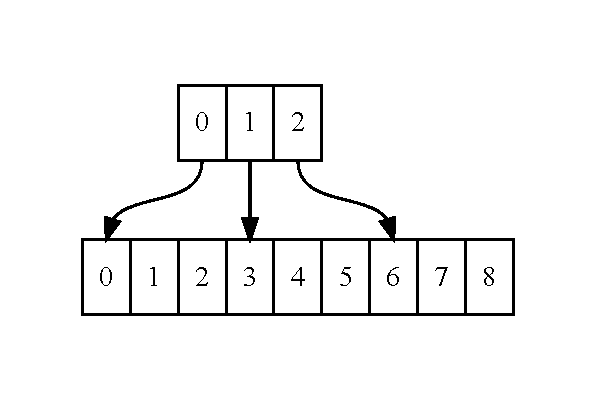
\includegraphics[scale=0.4]{float}
  }
  \caption{Représentation par tableaux}
\end{figure}

\begin{figure}[h]
  \centering{
    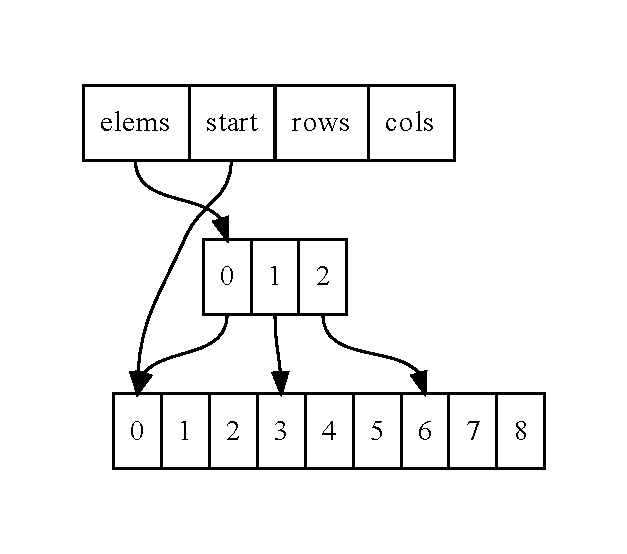
\includegraphics[scale=0.4]{matrix}
  }
  \caption{Représentation par structure}
\end{figure}

\section{Échange des lignes}

Afin d'accélérer la résolution du système, les échanges de lignes sont
faits en échangeant des pointeurs dans \emph{elems} plutôt que de
faire l'échange un-à-un des données.  Cela nous permet de faire un
échange de deux lignes en 3 étapes plutôt qu'en $3n$ étapes.


\end{document}
